\documentclass[12pt]{article}
\usepackage[utf8]{inputenc}
\usepackage[margin=1in]{geometry}
\usepackage{hyperref,indentfirst,amstext,amsmath,amssymb,amsthm,esint,float,graphicx,caption}

\usepackage[hyperref=true,backref=true,sorting=none]{biblatex}
\hypersetup{colorlinks=true,linkcolor=red,citecolor=red,urlcolor=blue}
\addbibresource{main.bib}
\renewcommand*{\bibfont}{\small}

\let\Pr\relax
\DeclareMathOperator*{\Pr}{\mathbb{P}}
\DeclareMathOperator*{\E}{\mathbb{E}}
\graphicspath{{./graphs/}}

\parindent 0.3in
\title{A Survey of Multi-Armed Bandit Learning}
\author{James Heppenstall, Haochen Li, Alberto Mizrahi}
\date{7 May 2019}

\begin{document}
\maketitle

\section{Introduction}

In this project, we focus on two formalizations of the multi-armed bandit problem: \textbf{stochastic iid rewards} and \textbf{adversarial rewards}. For the former, we survey epsilon strategies, UCB strategies, and Thompson sampling. For the latter, we survey the Exp3 and Exp3.P algorithms. In particular, we experimentally verify their regret bounds and compare their performance on Bernouilli trials and adversarial data. We finally motivate the problem in the broader context of Princeton's Theoretical Machine Learning (COS 511) course.

At a high level, the multi-armed bandit problem is a sequential decision problem concerned with how one dynamically allocates a resource among a set of actions to maximize some cumulative reward \cite{robbins1952}. While the original motivation for this problem came from clinical trials \cite{thompson1933}, the term ``multi-armed bandit" actually traces back to slot machines, each colloquially referred to as a ``one-armed bandit", by virtue of the arm one pulls down and the fact that they often empty gamblers' pockets. It should come as no surprise that Gittins' canonical example therefore considers a gambler who must decide which arm to pull among $K$ non-identical slot machines in order to maximize his return \cite{gittins1979}.

The multi-armed bandit learning problem has received much attention, particularly in the reinforcement learning community, because it touches upon the intrinsic tradeoff between \textbf{exploration} and \textbf{exploitation} in sequential experiments \cite{bubeck2012}. In the context of Gittins' slot machines, should one \textit{explore} slot machines with unknown rewards or \textit{exploit} the slot machine believed to give the highest reward? Every algorithm we survey approaches this fundamental question in a different manner, yielding varying theoretical guarantees and empirical results.

\section{Theoretical Background}

\subsection{Notation and Terminology}

We adopt Bubeck and Cesa-Bianchi's notation and terminology to formulate the multi-armed bandit problem \cite{bubeck2012}. Let the agent implementing some bandit strategy be the player. Assume there are $K\geq 2$ arms and $T\geq K$ rounds, both \textit{known} to the player. Each arm $i=1,...,K$ is associated with a sequence $X_{i,1},...,X_{i,T}$ of \textit{unknown} rewards. Every round $t=1,...,T$, the player selects an arm $I_{t}\in\{1,...,K\}$ and receives the reward $X_{I_{t},t}$. The goal is to maximize the player's cumulative reward $\sum_{t=1}^{T}X_{I_{t},t}$.

In the stochastic iid reward setting, each arm $i$ is associated with a probability distribution $\nu_{1},...,\nu_{K}$ that remains identical throughout. Every round $t$, the reward $X_{I_{t},t}\sim\nu_{I_{t}}$ is drawn independently of past player actions. In the adversarial reward setting, an adversary defines a gain vector $g_{t}=(g_{1,t},...,g_{K,t})$ at the beginning of every round $t$. The player then selects arm $I_{t}$ and receives the reward $X_{I_{t},t}=g_{I_{t},t}$ without observing the gains of the other arms. Note that stochastic iid rewards are a strict subset of adversarial rewards where the gain vector in round $t$ is defined according to random draws from $\nu_{1},...,\nu_{K}$.

The formulation above clearly mirrors the online learning problems\footnote{In fact, the formulation can be thought of as a simple version of online reinforcement learning.} we studied in COS 511, such as the variants of support vector machines \cite{lecture16} and gradient descent \cite{lecture18}. It is therefore natural to think about the theoretical guarantees of a bandit strategy in terms of \textbf{regret}; that is, its performance with respect to the optimal strategy. The regret after $T$ rounds is defined as
\begin{align}
R_{T}=\max_{i=1,...,K}\sum_{t=1}^{T}X_{i,t}-\sum_{t=1}^{T}X_{I_{t},t}.
\end{align}

With that said, player actions $I_{t}$ and rewards $X_{I_{t},t}$ are often assumed to be stochastic and so we introduce two further definitions of regret. The \textbf{expected regret} after $T$ rounds is defined as $\E[R_T]$ while the \textbf{pseudo-regret} is defined as 
\begin{gather}
\bar{R}_{T}=\max_{i=1,...,K}\E\Bigg{[}\sum_{t=1}^{T}X_{i,t}-\sum_{t=1}^{T}X_{I_{t},t}\Bigg{]}
\end{gather}
where expectation is taken with respect to random draws of both player actions and rewards. It is trivial that $\bar{R}_{T}\leq\E[R_{T}]$. In this project, we mainly provide upper bounds on the pseudo-regret because it is easier to reason about than the expected regret.

Before doing so, however, we cite the minimax lower bound without proof. Let $Y_{i,1},...,Y_{i,T}$ be a sequence of rewards associated with arm $i$ such that $Y_{i,t}\in\{0,1\}$ for all $t$. It follows that
\begin{align}
\inf\sup\Bigg{(}\max_{i=1,...,K}\E\Bigg{[}\sum_{i=1}^{T}Y_{i,t}-\sum_{i=1}^{T}Y_{I_{t},t}\Bigg{]}\Bigg{)}\geq\frac{1}{20}\sqrt{TK}
\end{align}
where the supremum is over all distributions of rewards and the infimum is over all player actions \cite{bubeck2012}. Since $\max_{i=1,..,K}\E[\sum_{i=1}^{T}Y_{i,t}-\sum_{i=1}^{T}Y_{I_{t},t}]=\bar{R}_{n}\leq\E[R_{n}]$, (3) provides a lower bound on the pseudo-regret, and by extension the expected regret.

\subsection{Epsilon Strategies}

The heart of the multi-armed bandit problem is the tradeoff between exploration and exploitation. Assuming stochastic iid rewards, a simple approach to this tradeoff is algorithms that behave somewhat greedily. That is, every round $t$, the player selects a uniformly random arm with probability $\epsilon_{t}$ and selects the arm with the highest observed mean reward with probability $1-\epsilon_{t}$. Epsilon strategies that binarily distinguish between exploration (uniformly random arms) and exploitation (the greedy choice) are called semi-uniform methods \cite{mohri2005}.

We first consider the \textbf{$\epsilon$-greedy algorithm} where $\epsilon_{t}=\epsilon$ for all $t$ and the \textbf{$\epsilon$-first algorithm} where $\epsilon_{t}=1$ for $t=1,...,\epsilon T$ and $\epsilon_{t}=0$ for $t=\epsilon T+1,...,T$. Here, $\epsilon\in[0,1]$ is a tunable hyperparameter that captures the tradeoff between exploration and exploitation \cite{sutton1998}. In other words, $\epsilon=0$ represents pure exploration and $\epsilon=1$ represents pure exploitation. To motivate an upper bound on the pseudo-regret, suppose the greedy choice in both strategies is the optimal arm. In this case, the player could still select a sub-optimal arm with probability $\epsilon$ (under $\epsilon$-greedy) or for $\epsilon T$ rounds (under $\epsilon$-first). This implies a \textit{linear} upper bound on the pseudo-regret of approximately $\epsilon T=\mathcal{O}(T)$ if $X_{i,t}\in[0,1]$. Intuitively, this occurs due to the constant value of $\epsilon_{t}$; that is, a constant amount of exploration ignorant of the round $t$\footnote{As an aside, though relevant to COS 511, it can be proven that the $\epsilon$-first algorithm, under the PAC framework, needs $\mathcal{O}\Big{(}\frac{K}{\alpha^{2}}\log\frac{K}{\delta}\Big{)}$ random selections to find an $\alpha$-optimal arm with probability $1-\delta$ \cite{evendar2002}.}.

A natural extension to the $\epsilon$-greedy and $\epsilon$-first algorithms, based on the notion of exploring first and exploiting later, is the \textbf{$\epsilon$-decreasing algorithm}. In this bandit strategy, $\epsilon_{t}=\min\{1,\epsilon_{0}\delta_{t}\}$ for all $t$ where $\epsilon_{0}>0$ and $\delta_{t}\in(0,1)$ are tunable hyperparameters \cite{sutton1998}. Assuming $\epsilon_{0}$ is relatively high (say $\epsilon_{0}\geq\frac{1}{2}$), we initially explore different arms while decreasing $\epsilon$ by a factor of $\delta_{t}$ every round, ultimately shifting from exploration (high $\epsilon_{t}$) to exploitation (low $\epsilon_{t}$). Clearly, $\epsilon_{t}$ is no longer constant but decreasing in this algorithm. Auer et al. prove that if $\epsilon_{0}=\frac{cK}{d^{2}}$ (where $c>0$ and $0<d<1$) and $\delta_{t}=\frac{1}{t}$ then the upper bound on the expected regret is $\mathcal{O}(\log T)$ \cite{auer2002}. This imples a \textit{logarithmic} upper bound on the pseudo-regret because $\bar{R}_{T}\leq\E[R_{T}]$, which is tight according to Lai and Robbins \cite{lai1985}.

\subsection{Upper Confidence Bound (UCB) Strategies}

We now consider a simple version of the \textbf{upper confidence bound (UCB) algorithm} \cite{auer2002}. At a high level, this strategy estimates the expected reward $\E[X_{i,t}]$ of each arm $i$ and \textit{optimistically} assumes our estimates are close to the truth. After an initial exploration phase, we select the arm with the highest estimate every round $t$. Depending on the observed reward, we recalibrate our estimate for said arm appropriately in what can be interpreted as the exploitation phase.

More formally, this strategy involves selecting each of the $K$ arms once, thereby providing initial estimates $\bar{X}_{i}$ of the expected reward of each arm $i$. Let $n_{i}$ denote the number of times $i$ has been selected thus far. Every subsequent round $t>K$, we then select the arm $i$ that maximizes $\bar{X}_{i}+\sqrt{2\log\frac{t}{n_{i}}}$. In keeping with notation, suppose $I_{t}$ is the arm selected in round $t$. After observing reward $X_{I_{t},t}$, we update
\begin{align}
\bar{X}_{I_{t}}\leftarrow\frac{n_{I_{t}}\bar{X}_{I_{t}}+X_{I_{t},t}}{n_{I_{t}}+1}\,\,\,\text{ followed by }\,\,\,n_{I_{t}}\leftarrow n_{I_{t}}+1.
\end{align}

Note that $\bar{X}_{i}+\sqrt{2\log\frac{t}{n_{i}}}$ defines an upper confidence bound for the expected reward of arm $i$. More so, the seemingly mysterious polylog term can be derived using Hoeffding's inequality, which was introduced in COS 511 \cite{lecture8}. Suppose $Y_{1},Y_{2},...,Y_{n_{i}}$ are the rewards generated by $i$ in each of its $n_{i}$ selections. Assume these rewards are stochastic iid such that $X_{i,t}\in[0,1]$. Let $Y=\frac{1}{n_{i}}\sum_{j=1}^{n_{i}}Y_{j}$ and $\mu=\E[Y_{1}]$. By Hoeffding's inequality, 
\begin{equation} 
Pr[Y\geq\mu+a]\leq e^{-2a^2 n_{i}}\,\,\,\text{ and }\,\,\,Pr[Y+a\leq\mu]\leq e^{-2a^2 n_{i}}
\end{equation}
where $a\geq 0$. Clearly, we want $Y$ to be less than or equal to $\mu+a$ with high probability. If we set $a=\sqrt{2\log\frac{t}{n_{i}}}$ then $Pr[Y \geq\mu+a]\leq t^{-4}$, which rapidly converges to $0$ as $t$ increases.

According to Auer et al., if the UCB algorithm is run on a multi-armed bandit problem with $K$ arms and stochastic iid rewards such that $X_{i,t}\in[0,1]$ then its pseudo-regret after $T$ rounds is at most $\mathcal{O}(\sqrt{KT\log T})$ \cite{auer2002}.

\subsection{Thompson Sampling}

\textbf{Thompson sampling} \cite{thompson1933} is another method to solve the multi-armed bandit problem. Our treatment of this algorithm is inspired by \cite{russo2018}. It differs fundamentally from the UCB algorithm because it uses a Bayesian approach\footnote{COS 511 covered Bayesian approaches to online learning with an introduction to Bayes' algorithm \cite{lecture21}.} to address the tradeoff between exploration and exploitation, while the UCB algorithm uses a frequentist's approach. In this project, we present a special version of Thompson sampling: the Beta-Bernouilli bandit.

Given $K$ arms, suppose arm $i$ generates a reward of $1$ with probability $\theta_{i}$ and a reward of $0$ with probability $1-\theta_{i}$. Note that each $\theta_{i}$ can be interpreted as the expected reward of $i$. Assume the expected rewards $\boldsymbol{\theta}=(\theta_{1}...,\theta_{K})$ are fixed (stochastic iid rewards). In the first round, the player selects arm $I_{1}$ and a reward $X_{I_{1},1}\in\{0,1\}$ is produced such that $\Pr[X_{I_{1},1}=1|I_{1},\mathbf{\theta}]=\theta_{I_{1}}$. After observing $X_{I_{1},1}$, the player updates his priors, selects another arm $I_{2}$, observes the reward $X_{I_{2},2}$, and the process continues.

Let the player start with independent priors over each $\theta_{i}$. Suppose these priors are beta-distributed with parameters $\boldsymbol{\alpha}=(\alpha_{1}, ..., \alpha_{K})$ and $\boldsymbol{\beta}=(\beta_{1}, ..., \beta_{K})$. In the first round, we set $\alpha_{i}=\beta_{i}=1$ for all $i=1,...,K$. Every round $t$, the player samples $\hat{\theta}_{i}\sim\text{Beta}(\alpha_{i},\beta_{i})$ for all $i$ and selects arm $I_{t}=\arg\max\hat{\theta}_{i}$. We then update the beta distributions according to Bayes' rule.
\begin{equation}
(\alpha_{i}, \beta_{i})\leftarrow
\begin{cases}
(\alpha_{i},\beta_{i})&\text{if}\ I_{t}\neq i \\
(\alpha_{i},\beta_{i})+(X_{I_{t},t},1-X_{I_{t},t})&\text{if}\ I_{t}=i
\end{cases}
\end{equation}
 
Note that a beta distribution with parameters $(\alpha_{i},\beta_{i})$ has mean $\frac{\alpha_{i}}{\alpha_{i}+\beta_{i}}$, which becomes more concentrated as $\alpha_{i}+\beta_{i}$ increases. Intuitively, Thompson sampling therefore applies Bayesian inference to shift from exploration (in earlier rounds) to exploitation (in later rounds) as the beta distributions of each prior become more concentrated. Although Thompson sampling is fundamentally different from the UCB algorithm, its pseudo-regret after $T$ rounds is also at most $\mathcal{O}(\sqrt{KT\log T})$ \cite{agrawal2012}.

\subsection{Exp3 and Exp3.P Algorithms}

Every bandit strategy outlined thus far has assumed stochastic iid rewards. This assumption has been at the core of the multi-armed bandit problem since the orginal formalization of Robbins \cite{robbins1952}. The \textbf{Exp3 algorithm}\footnote{Exp3 stands for ``exponential-weight algorithm for exploration and exploitation".}, however, makes no assumptions about the rewards; in the worst case, even adversarial rewards are permitted \cite{auer2003}. As a variant of Freund and Shapire's Hedge algorithm\footnote{This is loosely related to the multiplicative weights algorithm covered in COS 511 \cite{lecture16}.} \cite{freund1997}, this strategy initializes weights $w_{i}(1)=1$ for all $i=1,...,K$. Every round $t$, we define
\begin{align}
p_{i}(t)=(1-\gamma)\frac{w_{i}(t)}{\sum_{j=1}^{K}w_{j}(t)}+\frac{\gamma}{K}
\end{align}
for all $i$ and randomly select arm $I_{t}$ according to $p_{1}(t),...,p_{K}(t)$. After observing reward $X_{I_{t},t}$, we update $w_{I_{t}}(t+1)=w_{I_{t}}(t)\exp\Big{(}{\frac{\gamma}{K}\frac{X_{I_{t},t}}{p_{I_{t}}(t)}}\Big{)}$ and $w_{i}(t+1)=w_{i}(t)$ for all $i\neq I_{t}$. Here, $\gamma\in(0,1]$ is a tunable hyperparameter that captures the tradeoff between exploration and exploitation. In other words, small $\gamma$ represents high exploitation while $\gamma=1$ represents uniform exploration.

We cite an upper bound on the pseudo-regret of the Exp3 algorithm without proof. Assume $g\geq\max_{i=1,...,K}\sum_{t=1}^{T}X_{i,t}$ and $\gamma=\min\{1,\sqrt{\frac{K\ln K}{(e-1)g}}\}$ then $\bar{R}_{T}\leq 2\sqrt{e-1}\sqrt{gK\ln K}$ for any $T>0$ \cite{auer2003}. With that said, a major weakness of the Exp3 algorithm is the fact that the variance of the regret can be large. In fact, Auer et al. argue that this variance might be as large as $T^{\frac{3}{4}}$. This motivates a modified algorithm that controls said variance.

The \textbf{Exp3.P algorithm} initializes weights $w_{i}(1)=\exp\Big{(}\frac{\alpha\gamma}{3}\sqrt{\frac{T}{K}}\Big{)}$ for all $i=1,...,K$. It then takes the same steps as the Exp3 algorithm until the player observes reward $X_{I_{t},t}$. At this point, we update
\begin{align}
w_{I_{t}}(t+1)=w_{I_{t}}(t)\exp\Bigg{(}\frac{\gamma}{3K}\Bigg{(}\frac{X_{I_{t},t}}{p_{I_{t}}(t)}+\frac{\alpha}{p_{I_{t}}(t)\sqrt{KT}}\Bigg{)}\Bigg{)}
\end{align}
and $w_{i}(t+1)=w_{i}(t)\exp\Big{(}\frac{\alpha\gamma}{3K p_{i}(t)\sqrt{KT}}\Big{)}$ for all $i\neq I_{t}$. Clearly, $\alpha>0$ and $\gamma\in(0,1]$ are tunable hyperparamters. We refer the reader to Theorem 6.3 in \cite{auer2003} for a high probability upper bound on the regret, and by extension the pseudo-regret, of the Exp3.P algorithm.

\section{Empirical Results}

\subsection{Experimental Setup}

We initially tried to test our algorithms on stock data (i.e. each lever corresponds to a certain stock and at each round, the algorithm has to choose a stock that it believes will have the greatest return). However, this proved to be unsuccessful since stocks do not follow various of the assumptions of the algorithms, e.g the i.i.d of each lever (but see \cite{Shen:2015:PCO:2832249.2832384} for a possible workaround). Hence, instead opted to used generated data that did satisfy all the necessary assumptions. The data was generated as follows: a total of twenty levers were considered, each one following a Bernoulli distribution. The parameters of these twenty Bernoulli distributions were generated by the twenty numbers evenly space in the interval $[0.1, 0.9]$. At a round, the player chooses a lever which is modeled by some Bernoulli distribution with some parameter $p$; with probability $p$, the lever will return a reward of 1, and otherwise, it just returns 0.

Each algorithm was run for $T = 10,000$ rounds and each such experiment was repeated for 100 trials. The results per round where then averaged over all the trials and plotted along with a 99\% confidence interval.

In the stochastic setting, we expect that UCB, Thompson Sampling, and Epsilon strategies will outperform Exp3 algorithms because Exp3 algorithms are designed for an adversarial setting.

\subsection{Results}

\subsubsection{Epsilon Strategies}

Figure \ref{fig:epsilon-greedy-first} shows the results of running $\epsilon$-greedy and $\epsilon$-first under the setup specified in the above section.
\begin{figure}[H]
\begin{minipage}[h]{0.5\linewidth}
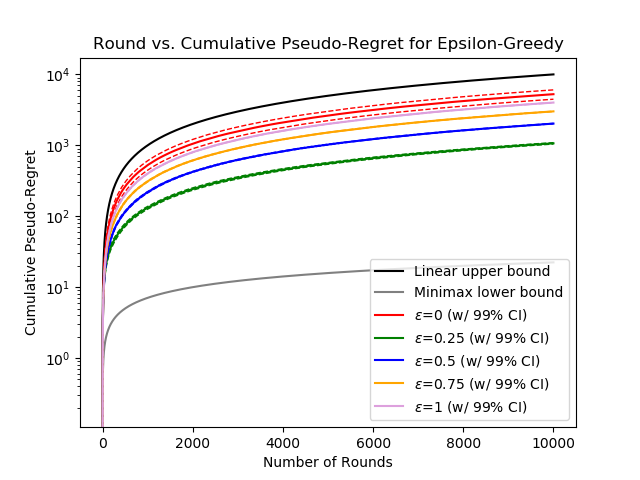
\includegraphics[width=\linewidth, height=0.75\linewidth]{epsilon-greedy.png}
\end{minipage}
\begin{minipage}[h]{0.5\linewidth}
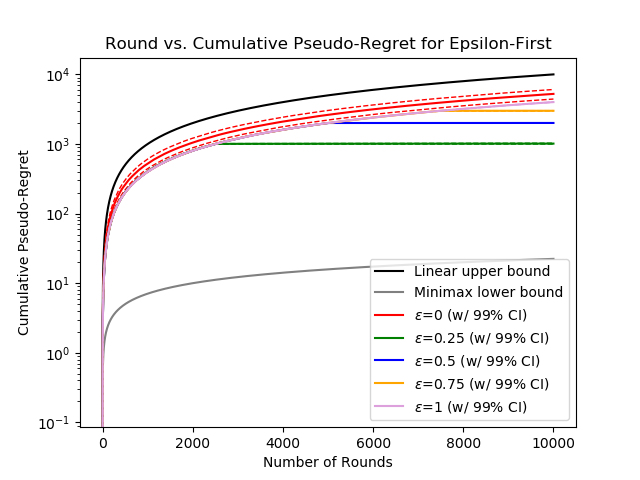
\includegraphics[width=\linewidth, height=0.75\linewidth]{epsilon-first.png}
\end{minipage}
\captionsetup{justification=centering}
\caption{Cumulative Regret vs Rounds for $\epsilon$-greedy and $\epsilon$-first.}
\label{fig:epsilon-greedy-first}
\end{figure}
Notice that both algorithms did very similar to each other and even the relative positions of the curves for the various epsilons were exactly the same for both algorithms. Furthermore, the graphs are very illuminating with respect to what is the optimal value of $\epsilon$, at least in our setting. Empirically, we clearly see that low exploration rates (or $\epsilon$) are preferable. This can be seen from the fact that an $\epsilon$ of 0.25 outperformed the one of $0.5$, and that one outperformed the one of $0.75$. Intuitively, this makes sense. Given that our setting does not have that many levers, the need for constant exploration is not that high. Even with a low $\epsilon$, given enough rounds, our algorithm is expected to have sampled the majority levers. Once this occurs, the algorithm will have a good approximate knowledge of which one is the best lever and the high exploitation rate (or $1-\epsilon$) will allow it to take advantage of that in many more occasions that in cases with higher $\epsilon$. Of course, if $\epsilon$ is too small (or as in our graph, it is zero), then exploration will not be done with enough consistency and this in turn will lead to less effective exploration and thus, higher regret. Finally, we notice that the worst case was when no exploration was done. This makes sense: the algorithm chose a random lever and pulled that one at every round. By simple probability, chances are the lever chosen was not the best one and hence, the algorithm will have high regrets. 

For empirically testing $\epsilon$-decreasing, we initialized $\epsilon=0.5$ (which evenly balances exploration and exploitation) and we tested for various decreasing factors $\delta$. Furthermore, we did this decrease every $N=1000$ rounds. The results are shown in Figure \ref{fig:epsilon-decreasing}.
\begin{figure}
\begin{center}
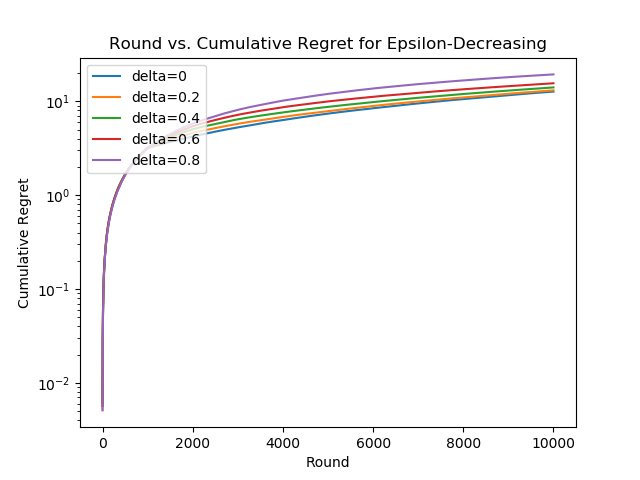
\includegraphics[scale=0.75]{epsilon-decreasing.png}
  \captionsetup{justification=centering}
  \caption{Cumulative Regret vs Rounds for $\epsilon$-decreasing with $\epsilon=0.5$ and $N=1000$.}
  \label{fig:epsilon-decreasing}
 \end{center}
\end{figure}
It can be seen that the lower the decreasing factor, the better the algorithm approximately performed. Intuitively, this makes sense for the following reason. Our initial $\epsilon$ is high and it is not modified until after 1000 rounds. It can thus be expected that by that round, the algorithm has explored enough to the point that it found a well performing lever. Hence, there is little need for more exploration and thus, substantially decreasing $\epsilon$ (or even setting it to 0 as in $\delta=0$), permits the algorithm to perform more exploitation.

\subsection{UCB and Thompson Sampling}

\textbf{Thompson Sampling Final Mean Pseudo Regret $105.12$, UCB Final Mean Pseudo Regret $753.12$}

We plot the upper bound and lower bound for UCB and Thompson Sampling. We also plot the mean pseudo-regret for both algorithms with $99$\% confidence interval.As the graph shows, the performance of UCB algorithm and Thompson Sampling algorithm fall between the theoretical upper bound and lower bound. Although the upper bound and lower bound are not very tight. Furthermore, Thompson sampling outperforms UCB algorithm by a significant margin despite the fact that both algorithms have the same theoretical lower bound and upper bound. These results show that theory can often provide very good qualitative information about performance of algorithms, but not very good quantitative information.

\begin{figure}[tb]
  \includegraphics[width=\linewidth]{Pseudo-Regret-Bounds.png}
  \captionsetup{justification=centering}
  \caption{Stochastic Reward Setting Pseudo-Regret Bounds}
\end{figure}

\subsection{Exp3 and Exp3.P Algorithms}

\begin{figure}[H]
\begin{minipage}[h]{0.5\linewidth}
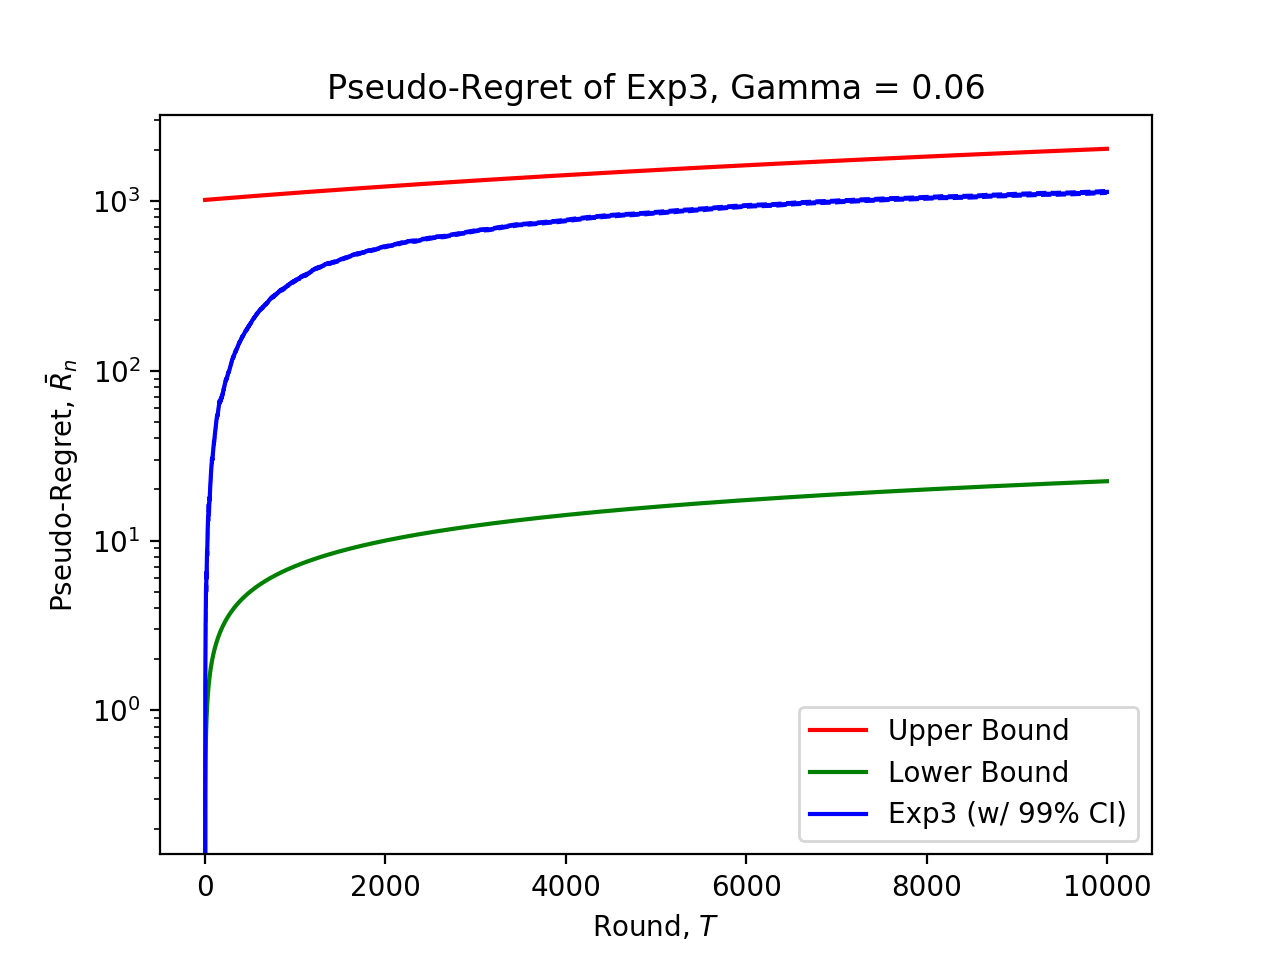
\includegraphics[width=\linewidth, height=0.75\linewidth]{exp3-1.png}
\end{minipage}
\begin{minipage}[h]{0.5\linewidth}
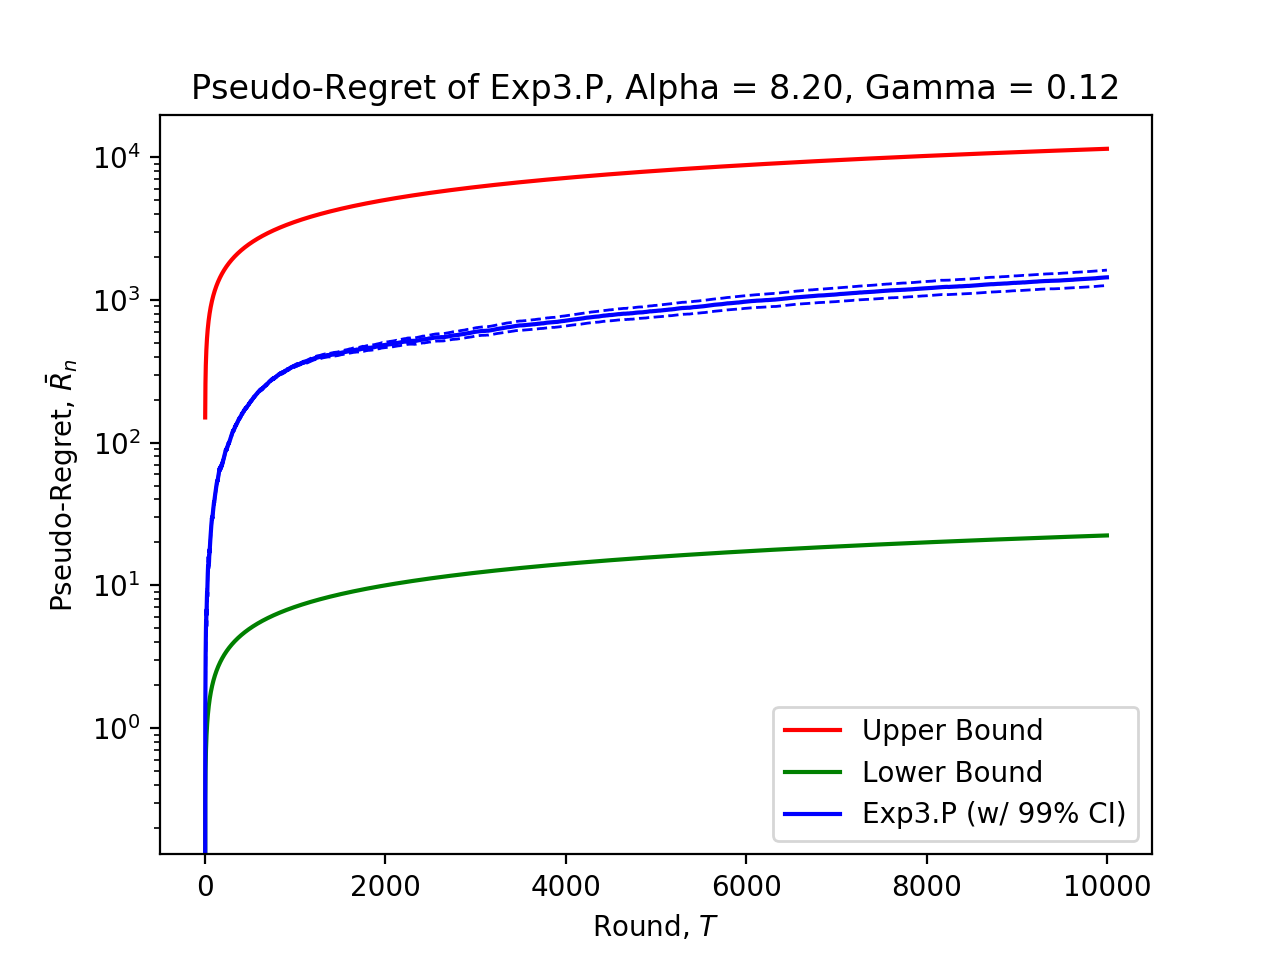
\includegraphics[width=\linewidth, height=0.75\linewidth]{exp3P-1.png}
\end{minipage}
\end{figure}

\section{Conclusion}

\newpage
\printbibliography

\end{document}